% Graphic for TeX using PGF
% Title: /home/merelas/Bureau/ngreen/article/figures/BBU2.dia
% Creator: Dia v0.97.3
% CreationDate: Fri Feb 10 16:39:12 2017
% For: merelas
% \usepackage{tikz}
% The following commands are not supported in PSTricks at present
% We define them conditionally, so when they are implemented,
% this pgf file will use them.
\ifx\du\undefined
  \newlength{\du}
\fi
\setlength{\du}{15\unitlength}
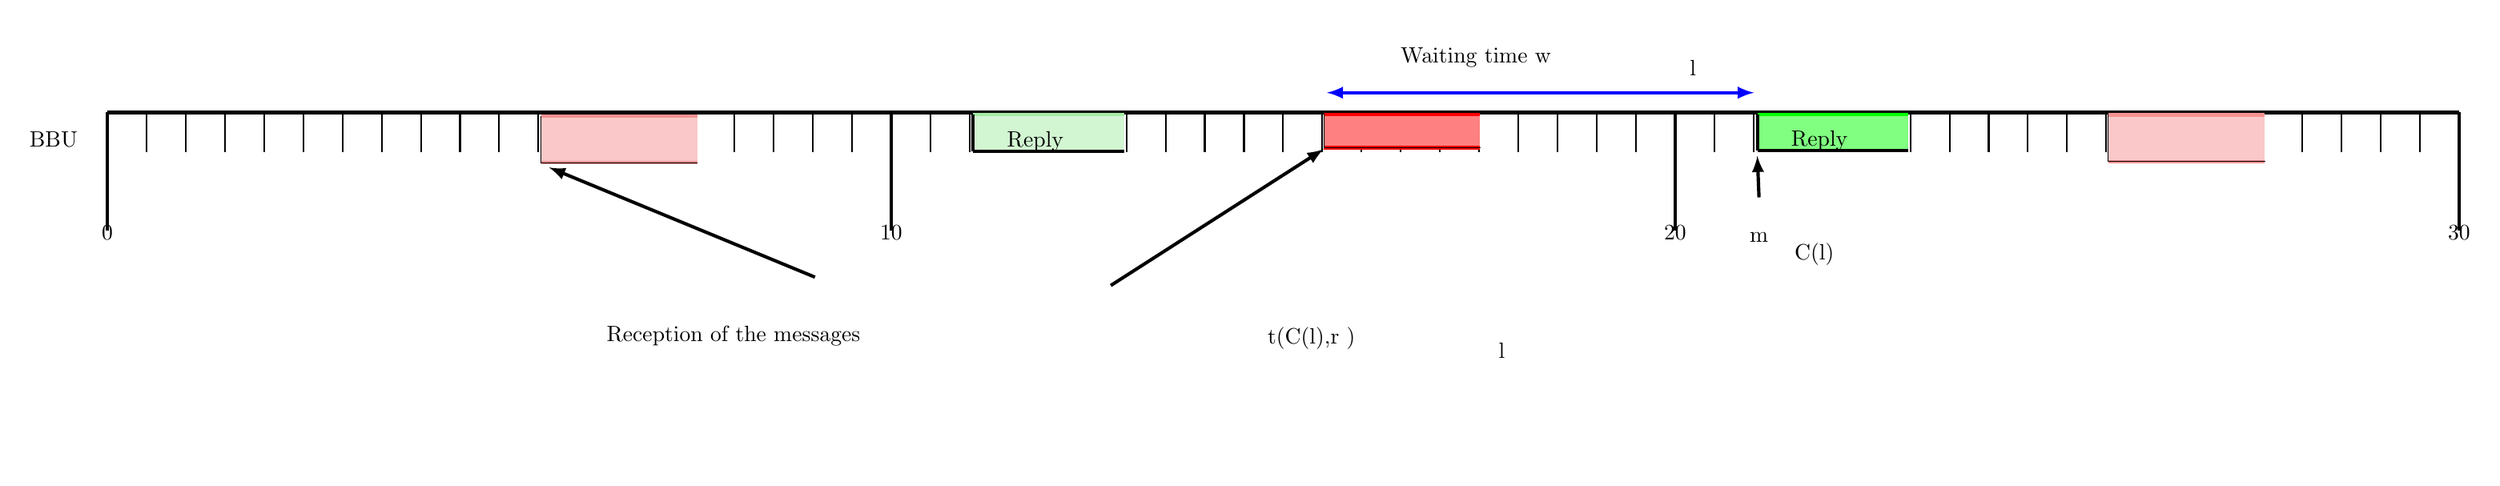
\begin{tikzpicture}
\pgftransformxscale{1.000000}
\pgftransformyscale{-1.000000}
\definecolor{dialinecolor}{rgb}{0.000000, 0.000000, 0.000000}
\pgfsetstrokecolor{dialinecolor}
\definecolor{dialinecolor}{rgb}{1.000000, 1.000000, 1.000000}
\pgfsetfillcolor{dialinecolor}
\pgfsetdash{}{0pt}
\pgfsetmiterjoin
% setfont left to latex
\pgfsetlinewidth{0.050000\du}
\definecolor{dialinecolor}{rgb}{0.000000, 0.000000, 0.000000}
\pgfsetstrokecolor{dialinecolor}
\draw (10.660000\du,6.845000\du)--(10.660000\du,8.028333\du);
\definecolor{dialinecolor}{rgb}{0.000000, 0.000000, 0.000000}
\pgfsetstrokecolor{dialinecolor}
\draw (11.839167\du,6.845000\du)--(11.839167\du,8.028333\du);
\definecolor{dialinecolor}{rgb}{0.000000, 0.000000, 0.000000}
\pgfsetstrokecolor{dialinecolor}
\draw (13.018333\du,6.845000\du)--(13.018333\du,8.028333\du);
\definecolor{dialinecolor}{rgb}{0.000000, 0.000000, 0.000000}
\pgfsetstrokecolor{dialinecolor}
\draw (14.197500\du,6.845000\du)--(14.197500\du,8.028333\du);
\definecolor{dialinecolor}{rgb}{0.000000, 0.000000, 0.000000}
\pgfsetstrokecolor{dialinecolor}
\draw (15.376667\du,6.845000\du)--(15.376667\du,8.028333\du);
\definecolor{dialinecolor}{rgb}{0.000000, 0.000000, 0.000000}
\pgfsetstrokecolor{dialinecolor}
\draw (16.555833\du,6.845000\du)--(16.555833\du,8.028333\du);
\definecolor{dialinecolor}{rgb}{0.000000, 0.000000, 0.000000}
\pgfsetstrokecolor{dialinecolor}
\draw (17.735000\du,6.845000\du)--(17.735000\du,8.028333\du);
\definecolor{dialinecolor}{rgb}{0.000000, 0.000000, 0.000000}
\pgfsetstrokecolor{dialinecolor}
\draw (18.914167\du,6.845000\du)--(18.914167\du,8.028333\du);
\definecolor{dialinecolor}{rgb}{0.000000, 0.000000, 0.000000}
\pgfsetstrokecolor{dialinecolor}
\draw (20.093333\du,6.845000\du)--(20.093333\du,8.028333\du);
\definecolor{dialinecolor}{rgb}{0.000000, 0.000000, 0.000000}
\pgfsetstrokecolor{dialinecolor}
\draw (21.272500\du,6.845000\du)--(21.272500\du,8.028333\du);
\definecolor{dialinecolor}{rgb}{0.000000, 0.000000, 0.000000}
\pgfsetstrokecolor{dialinecolor}
\draw (22.451667\du,6.845000\du)--(22.451667\du,8.028333\du);
\definecolor{dialinecolor}{rgb}{0.000000, 0.000000, 0.000000}
\pgfsetstrokecolor{dialinecolor}
\draw (23.630833\du,6.845000\du)--(23.630833\du,8.028333\du);
\definecolor{dialinecolor}{rgb}{0.000000, 0.000000, 0.000000}
\pgfsetstrokecolor{dialinecolor}
\draw (24.810000\du,6.845000\du)--(24.810000\du,8.028333\du);
\definecolor{dialinecolor}{rgb}{0.000000, 0.000000, 0.000000}
\pgfsetstrokecolor{dialinecolor}
\draw (25.989167\du,6.845000\du)--(25.989167\du,8.028333\du);
\definecolor{dialinecolor}{rgb}{0.000000, 0.000000, 0.000000}
\pgfsetstrokecolor{dialinecolor}
\draw (27.168333\du,6.845000\du)--(27.168333\du,8.028333\du);
\definecolor{dialinecolor}{rgb}{0.000000, 0.000000, 0.000000}
\pgfsetstrokecolor{dialinecolor}
\draw (28.347500\du,6.845000\du)--(28.347500\du,8.028333\du);
\definecolor{dialinecolor}{rgb}{0.000000, 0.000000, 0.000000}
\pgfsetstrokecolor{dialinecolor}
\draw (29.526667\du,6.845000\du)--(29.526667\du,8.028333\du);
\definecolor{dialinecolor}{rgb}{0.000000, 0.000000, 0.000000}
\pgfsetstrokecolor{dialinecolor}
\draw (30.705833\du,6.845000\du)--(30.705833\du,8.028333\du);
\definecolor{dialinecolor}{rgb}{0.000000, 0.000000, 0.000000}
\pgfsetstrokecolor{dialinecolor}
\draw (31.885000\du,6.845000\du)--(31.885000\du,8.028333\du);
\definecolor{dialinecolor}{rgb}{0.000000, 0.000000, 0.000000}
\pgfsetstrokecolor{dialinecolor}
\draw (33.064167\du,6.845000\du)--(33.064167\du,8.028333\du);
\definecolor{dialinecolor}{rgb}{0.000000, 0.000000, 0.000000}
\pgfsetstrokecolor{dialinecolor}
\draw (34.243333\du,6.845000\du)--(34.243333\du,8.028333\du);
\definecolor{dialinecolor}{rgb}{0.000000, 0.000000, 0.000000}
\pgfsetstrokecolor{dialinecolor}
\draw (35.422500\du,6.845000\du)--(35.422500\du,8.028333\du);
\definecolor{dialinecolor}{rgb}{0.000000, 0.000000, 0.000000}
\pgfsetstrokecolor{dialinecolor}
\draw (36.601667\du,6.845000\du)--(36.601667\du,8.028333\du);
\definecolor{dialinecolor}{rgb}{0.000000, 0.000000, 0.000000}
\pgfsetstrokecolor{dialinecolor}
\draw (37.780833\du,6.845000\du)--(37.780833\du,8.028333\du);
\definecolor{dialinecolor}{rgb}{0.000000, 0.000000, 0.000000}
\pgfsetstrokecolor{dialinecolor}
\draw (38.960000\du,6.845000\du)--(38.960000\du,8.028333\du);
\definecolor{dialinecolor}{rgb}{0.000000, 0.000000, 0.000000}
\pgfsetstrokecolor{dialinecolor}
\draw (40.139167\du,6.845000\du)--(40.139167\du,8.028333\du);
\definecolor{dialinecolor}{rgb}{0.000000, 0.000000, 0.000000}
\pgfsetstrokecolor{dialinecolor}
\draw (41.318333\du,6.845000\du)--(41.318333\du,8.028333\du);
\definecolor{dialinecolor}{rgb}{0.000000, 0.000000, 0.000000}
\pgfsetstrokecolor{dialinecolor}
\draw (42.497500\du,6.845000\du)--(42.497500\du,8.028333\du);
\definecolor{dialinecolor}{rgb}{0.000000, 0.000000, 0.000000}
\pgfsetstrokecolor{dialinecolor}
\draw (43.676667\du,6.845000\du)--(43.676667\du,8.028333\du);
\definecolor{dialinecolor}{rgb}{0.000000, 0.000000, 0.000000}
\pgfsetstrokecolor{dialinecolor}
\draw (44.855833\du,6.845000\du)--(44.855833\du,8.028333\du);
\definecolor{dialinecolor}{rgb}{0.000000, 0.000000, 0.000000}
\pgfsetstrokecolor{dialinecolor}
\draw (46.035000\du,6.845000\du)--(46.035000\du,8.028333\du);
\definecolor{dialinecolor}{rgb}{0.000000, 0.000000, 0.000000}
\pgfsetstrokecolor{dialinecolor}
\draw (47.214167\du,6.845000\du)--(47.214167\du,8.028333\du);
\definecolor{dialinecolor}{rgb}{0.000000, 0.000000, 0.000000}
\pgfsetstrokecolor{dialinecolor}
\draw (48.393333\du,6.845000\du)--(48.393333\du,8.028333\du);
\definecolor{dialinecolor}{rgb}{0.000000, 0.000000, 0.000000}
\pgfsetstrokecolor{dialinecolor}
\draw (49.572500\du,6.845000\du)--(49.572500\du,8.028333\du);
\definecolor{dialinecolor}{rgb}{0.000000, 0.000000, 0.000000}
\pgfsetstrokecolor{dialinecolor}
\draw (50.751667\du,6.845000\du)--(50.751667\du,8.028333\du);
\definecolor{dialinecolor}{rgb}{0.000000, 0.000000, 0.000000}
\pgfsetstrokecolor{dialinecolor}
\draw (51.930833\du,6.845000\du)--(51.930833\du,8.028333\du);
\definecolor{dialinecolor}{rgb}{0.000000, 0.000000, 0.000000}
\pgfsetstrokecolor{dialinecolor}
\draw (53.110000\du,6.845000\du)--(53.110000\du,8.028333\du);
\definecolor{dialinecolor}{rgb}{0.000000, 0.000000, 0.000000}
\pgfsetstrokecolor{dialinecolor}
\draw (54.289167\du,6.845000\du)--(54.289167\du,8.028333\du);
\definecolor{dialinecolor}{rgb}{0.000000, 0.000000, 0.000000}
\pgfsetstrokecolor{dialinecolor}
\draw (55.468333\du,6.845000\du)--(55.468333\du,8.028333\du);
\definecolor{dialinecolor}{rgb}{0.000000, 0.000000, 0.000000}
\pgfsetstrokecolor{dialinecolor}
\draw (56.647500\du,6.845000\du)--(56.647500\du,8.028333\du);
\definecolor{dialinecolor}{rgb}{0.000000, 0.000000, 0.000000}
\pgfsetstrokecolor{dialinecolor}
\draw (57.826667\du,6.845000\du)--(57.826667\du,8.028333\du);
\definecolor{dialinecolor}{rgb}{0.000000, 0.000000, 0.000000}
\pgfsetstrokecolor{dialinecolor}
\draw (59.005833\du,6.845000\du)--(59.005833\du,8.028333\du);
\definecolor{dialinecolor}{rgb}{0.000000, 0.000000, 0.000000}
\pgfsetstrokecolor{dialinecolor}
\draw (60.185000\du,6.845000\du)--(60.185000\du,8.028333\du);
\definecolor{dialinecolor}{rgb}{0.000000, 0.000000, 0.000000}
\pgfsetstrokecolor{dialinecolor}
\draw (61.364167\du,6.845000\du)--(61.364167\du,8.028333\du);
\definecolor{dialinecolor}{rgb}{0.000000, 0.000000, 0.000000}
\pgfsetstrokecolor{dialinecolor}
\draw (62.543333\du,6.845000\du)--(62.543333\du,8.028333\du);
\definecolor{dialinecolor}{rgb}{0.000000, 0.000000, 0.000000}
\pgfsetstrokecolor{dialinecolor}
\draw (63.722500\du,6.845000\du)--(63.722500\du,8.028333\du);
\definecolor{dialinecolor}{rgb}{0.000000, 0.000000, 0.000000}
\pgfsetstrokecolor{dialinecolor}
\draw (64.901667\du,6.845000\du)--(64.901667\du,8.028333\du);
\definecolor{dialinecolor}{rgb}{0.000000, 0.000000, 0.000000}
\pgfsetstrokecolor{dialinecolor}
\draw (66.080833\du,6.845000\du)--(66.080833\du,8.028333\du);
\definecolor{dialinecolor}{rgb}{0.000000, 0.000000, 0.000000}
\pgfsetstrokecolor{dialinecolor}
\draw (67.260000\du,6.845000\du)--(67.260000\du,8.028333\du);
\definecolor{dialinecolor}{rgb}{0.000000, 0.000000, 0.000000}
\pgfsetstrokecolor{dialinecolor}
\draw (68.439167\du,6.845000\du)--(68.439167\du,8.028333\du);
\definecolor{dialinecolor}{rgb}{0.000000, 0.000000, 0.000000}
\pgfsetstrokecolor{dialinecolor}
\draw (69.618333\du,6.845000\du)--(69.618333\du,8.028333\du);
\definecolor{dialinecolor}{rgb}{0.000000, 0.000000, 0.000000}
\pgfsetstrokecolor{dialinecolor}
\draw (70.797500\du,6.845000\du)--(70.797500\du,8.028333\du);
\definecolor{dialinecolor}{rgb}{0.000000, 0.000000, 0.000000}
\pgfsetstrokecolor{dialinecolor}
\draw (71.976667\du,6.845000\du)--(71.976667\du,8.028333\du);
\definecolor{dialinecolor}{rgb}{0.000000, 0.000000, 0.000000}
\pgfsetstrokecolor{dialinecolor}
\draw (73.155833\du,6.845000\du)--(73.155833\du,8.028333\du);
\definecolor{dialinecolor}{rgb}{0.000000, 0.000000, 0.000000}
\pgfsetstrokecolor{dialinecolor}
\draw (74.335000\du,6.845000\du)--(74.335000\du,8.028333\du);
\definecolor{dialinecolor}{rgb}{0.000000, 0.000000, 0.000000}
\pgfsetstrokecolor{dialinecolor}
\draw (75.514167\du,6.845000\du)--(75.514167\du,8.028333\du);
\definecolor{dialinecolor}{rgb}{0.000000, 0.000000, 0.000000}
\pgfsetstrokecolor{dialinecolor}
\draw (76.693333\du,6.845000\du)--(76.693333\du,8.028333\du);
\definecolor{dialinecolor}{rgb}{0.000000, 0.000000, 0.000000}
\pgfsetstrokecolor{dialinecolor}
\draw (77.872500\du,6.845000\du)--(77.872500\du,8.028333\du);
\definecolor{dialinecolor}{rgb}{0.000000, 0.000000, 0.000000}
\pgfsetstrokecolor{dialinecolor}
\draw (79.051667\du,6.845000\du)--(79.051667\du,8.028333\du);
\definecolor{dialinecolor}{rgb}{0.000000, 0.000000, 0.000000}
\pgfsetstrokecolor{dialinecolor}
\draw (80.230833\du,6.845000\du)--(80.230833\du,8.028333\du);
\definecolor{dialinecolor}{rgb}{0.000000, 0.000000, 0.000000}
\pgfsetstrokecolor{dialinecolor}
\draw (81.410000\du,6.845000\du)--(81.410000\du,8.028333\du);
\pgfsetlinewidth{0.100000\du}
\definecolor{dialinecolor}{rgb}{0.000000, 0.000000, 0.000000}
\pgfsetstrokecolor{dialinecolor}
\draw (10.660000\du,6.845000\du)--(10.660000\du,10.395000\du);
\definecolor{dialinecolor}{rgb}{0.000000, 0.000000, 0.000000}
\pgfsetstrokecolor{dialinecolor}
\node at (10.660000\du,10.470000\du){0};
\definecolor{dialinecolor}{rgb}{0.000000, 0.000000, 0.000000}
\pgfsetstrokecolor{dialinecolor}
\draw (34.243333\du,6.845000\du)--(34.243333\du,10.395000\du);
\definecolor{dialinecolor}{rgb}{0.000000, 0.000000, 0.000000}
\pgfsetstrokecolor{dialinecolor}
\node at (34.243333\du,10.470000\du){10};
\definecolor{dialinecolor}{rgb}{0.000000, 0.000000, 0.000000}
\pgfsetstrokecolor{dialinecolor}
\draw (57.826667\du,6.845000\du)--(57.826667\du,10.395000\du);
\definecolor{dialinecolor}{rgb}{0.000000, 0.000000, 0.000000}
\pgfsetstrokecolor{dialinecolor}
\node at (57.826667\du,10.470000\du){20};
\definecolor{dialinecolor}{rgb}{0.000000, 0.000000, 0.000000}
\pgfsetstrokecolor{dialinecolor}
\draw (81.410000\du,6.845000\du)--(81.410000\du,10.395000\du);
\definecolor{dialinecolor}{rgb}{0.000000, 0.000000, 0.000000}
\pgfsetstrokecolor{dialinecolor}
\node at (81.410000\du,10.470000\du){30};
\definecolor{dialinecolor}{rgb}{0.000000, 0.000000, 0.000000}
\pgfsetstrokecolor{dialinecolor}
\draw (10.660000\du,6.845000\du)--(81.410000\du,6.845000\du);
% setfont left to latex
\definecolor{dialinecolor}{rgb}{0.000000, 0.000000, 0.000000}
\pgfsetstrokecolor{dialinecolor}
\node[anchor=west] at (28.310000\du,6.395000\du){};
% setfont left to latex
\definecolor{dialinecolor}{rgb}{0.000000, 0.000000, 0.000000}
\pgfsetstrokecolor{dialinecolor}
\node[anchor=west] at (8.050000\du,7.650000\du){BBU};
\pgfsetmiterjoin
\pgfsetdash{{\pgflinewidth}{0.200000\du}}{0cm}
\pgfsetlinewidth{0.000000\du}
\definecolor{dialinecolor}{rgb}{0.500000, 0.500000, 0.500000}
\pgfsetstrokecolor{dialinecolor}
\draw (47.260000\du,6.905000\du)--(51.960000\du,6.905000\du);
\pgfsetmiterjoin
\pgfsetdash{}{0pt}
\pgfsetlinewidth{0.100000\du}
\definecolor{dialinecolor}{rgb}{1.000000, 0.500000, 0.500000}
\pgfsetfillcolor{dialinecolor}
\fill (47.260000\du,7.905000\du)--(47.260000\du,6.905000\du)--(51.960000\du,6.905000\du)--(51.960000\du,7.905000\du)--cycle;
\pgfsetmiterjoin
\pgfsetdash{}{0pt}
\pgfsetlinewidth{0.100000\du}
\definecolor{dialinecolor}{rgb}{1.000000, 0.000000, 0.000000}
\pgfsetstrokecolor{dialinecolor}
\draw (47.260000\du,6.905000\du)--(51.960000\du,6.905000\du);
\definecolor{dialinecolor}{rgb}{1.000000, 0.000000, 0.000000}
\pgfsetstrokecolor{dialinecolor}
\draw (47.260000\du,7.905000\du)--(51.960000\du,7.905000\du);
\pgfsetdash{}{0pt}
\pgfsetlinewidth{0.000000\du}
\definecolor{dialinecolor}{rgb}{0.000000, 0.000000, 0.000000}
\pgfsetstrokecolor{dialinecolor}
\draw (47.260000\du,7.905000\du)--(51.960000\du,7.905000\du);
\definecolor{dialinecolor}{rgb}{0.000000, 0.000000, 0.000000}
\pgfsetstrokecolor{dialinecolor}
\draw (47.260000\du,7.905000\du)--(47.260000\du,6.905000\du);
% setfont left to latex
\definecolor{dialinecolor}{rgb}{0.000000, 0.000000, 0.000000}
\pgfsetstrokecolor{dialinecolor}
\node[anchor=east] at (47.260000\du,7.658497\du){};
\pgfsetmiterjoin
\pgfsetdash{{\pgflinewidth}{0.200000\du}}{0cm}
\pgfsetlinewidth{0.100000\du}
\definecolor{dialinecolor}{rgb}{0.500000, 0.500000, 0.500000}
\pgfsetstrokecolor{dialinecolor}
\draw (60.300000\du,6.900000\du)--(64.850000\du,6.900000\du);
\pgfsetmiterjoin
\pgfsetdash{}{0pt}
\pgfsetlinewidth{0.100000\du}
\definecolor{dialinecolor}{rgb}{0.500000, 1.000000, 0.500000}
\pgfsetfillcolor{dialinecolor}
\fill (60.300000\du,8.000000\du)--(60.300000\du,6.900000\du)--(64.850000\du,6.900000\du)--(64.850000\du,8.000000\du)--cycle;
\pgfsetmiterjoin
\pgfsetdash{}{0pt}
\pgfsetlinewidth{0.100000\du}
\definecolor{dialinecolor}{rgb}{0.000000, 1.000000, 0.000000}
\pgfsetstrokecolor{dialinecolor}
\draw (60.300000\du,6.900000\du)--(64.850000\du,6.900000\du);
\pgfsetdash{}{0pt}
\pgfsetlinewidth{0.100000\du}
\definecolor{dialinecolor}{rgb}{0.000000, 0.000000, 0.000000}
\pgfsetstrokecolor{dialinecolor}
\draw (60.300000\du,8.000000\du)--(64.850000\du,8.000000\du);
\definecolor{dialinecolor}{rgb}{0.000000, 0.000000, 0.000000}
\pgfsetstrokecolor{dialinecolor}
\draw (60.300000\du,8.000000\du)--(60.300000\du,6.900000\du);
% setfont left to latex
\definecolor{dialinecolor}{rgb}{0.000000, 0.000000, 0.000000}
\pgfsetstrokecolor{dialinecolor}
\node[anchor=east] at (60.200000\du,7.750000\du){};
% setfont left to latex
\definecolor{dialinecolor}{rgb}{0.000000, 0.000000, 0.000000}
\pgfsetstrokecolor{dialinecolor}
\node[anchor=west] at (61.050000\du,7.700000\du){Reply};
\pgfsetlinewidth{0.100000\du}
\pgfsetdash{}{0pt}
\pgfsetdash{}{0pt}
\pgfsetbuttcap
{
\definecolor{dialinecolor}{rgb}{0.000000, 0.000000, 1.000000}
\pgfsetfillcolor{dialinecolor}
% was here!!!
\pgfsetarrowsstart{latex}
\pgfsetarrowsend{latex}
\definecolor{dialinecolor}{rgb}{0.000000, 0.000000, 1.000000}
\pgfsetstrokecolor{dialinecolor}
\draw (47.350000\du,6.250000\du)--(60.200000\du,6.250000\du);
}
% setfont left to latex
\definecolor{dialinecolor}{rgb}{0.000000, 0.000000, 0.000000}
\pgfsetstrokecolor{dialinecolor}
\node[anchor=west] at (53.250000\du,12.300000\du){};
% setfont left to latex
\definecolor{dialinecolor}{rgb}{0.000000, 0.000000, 0.000000}
\pgfsetstrokecolor{dialinecolor}
\node[anchor=west] at (59.800000\du,10.600000\du){m};
% setfont left to latex
\definecolor{dialinecolor}{rgb}{0.000000, 0.000000, 0.000000}
\pgfsetstrokecolor{dialinecolor}
\node[anchor=west] at (59.800000\du,12.363889\du){};
\pgfsetlinewidth{0.100000\du}
\pgfsetdash{}{0pt}
\pgfsetdash{}{0pt}
\pgfsetbuttcap
{
\definecolor{dialinecolor}{rgb}{0.000000, 0.000000, 0.000000}
\pgfsetfillcolor{dialinecolor}
% was here!!!
\pgfsetarrowsend{latex}
\definecolor{dialinecolor}{rgb}{0.000000, 0.000000, 0.000000}
\pgfsetstrokecolor{dialinecolor}
\draw (60.350000\du,9.400000\du)--(60.300000\du,8.150000\du);
}
% setfont left to latex
\definecolor{dialinecolor}{rgb}{0.000000, 0.000000, 0.000000}
\pgfsetstrokecolor{dialinecolor}
\node[anchor=west] at (57.800000\du,4.350000\du){};
% setfont left to latex
\definecolor{dialinecolor}{rgb}{0.000000, 0.000000, 0.000000}
\pgfsetstrokecolor{dialinecolor}
\node[anchor=west] at (52.250000\du,14.000000\du){l};
\pgfsetlinewidth{0.100000\du}
\pgfsetdash{}{0pt}
\pgfsetdash{}{0pt}
\pgfsetbuttcap
{
\definecolor{dialinecolor}{rgb}{0.000000, 0.000000, 0.000000}
\pgfsetfillcolor{dialinecolor}
% was here!!!
\pgfsetarrowsend{latex}
\definecolor{dialinecolor}{rgb}{0.000000, 0.000000, 0.000000}
\pgfsetstrokecolor{dialinecolor}
\draw (40.850000\du,12.050000\du)--(47.250000\du,7.950000\du);
}
% setfont left to latex
\definecolor{dialinecolor}{rgb}{0.000000, 0.000000, 0.000000}
\pgfsetstrokecolor{dialinecolor}
\node[anchor=west] at (56.350000\du,5.200000\du){};
% setfont left to latex
\definecolor{dialinecolor}{rgb}{0.000000, 0.000000, 1.000000}
\pgfsetstrokecolor{dialinecolor}
\node[anchor=west] at (49.300000\du,5.200000\du){Waiting time w};
% setfont left to latex
\definecolor{dialinecolor}{rgb}{0.000000, 0.000000, 1.000000}
\pgfsetstrokecolor{dialinecolor}
\node[anchor=west] at (58.000000\du,5.500000\du){l};
% setfont left to latex
\definecolor{dialinecolor}{rgb}{0.000000, 0.000000, 1.000000}
\pgfsetstrokecolor{dialinecolor}
\node[anchor=west] at (58.000000\du,6.558333\du){};
% setfont left to latex
\definecolor{dialinecolor}{rgb}{0.000000, 0.000000, 0.000000}
\pgfsetstrokecolor{dialinecolor}
\node[anchor=west] at (45.300000\du,13.650000\du){t(C(l),r )};
% setfont left to latex
\definecolor{dialinecolor}{rgb}{0.000000, 0.000000, 0.000000}
\pgfsetstrokecolor{dialinecolor}
\node[anchor=west] at (45.300000\du,15.413889\du){};
% setfont left to latex
\definecolor{dialinecolor}{rgb}{0.000000, 0.000000, 0.000000}
\pgfsetstrokecolor{dialinecolor}
\node[anchor=west] at (45.300000\du,17.177778\du){};
% setfont left to latex
\definecolor{dialinecolor}{rgb}{0.000000, 0.000000, 0.000000}
\pgfsetstrokecolor{dialinecolor}
\node[anchor=west] at (61.600000\du,10.850000\du){};
% setfont left to latex
\definecolor{dialinecolor}{rgb}{0.000000, 0.000000, 0.000000}
\pgfsetstrokecolor{dialinecolor}
\node[anchor=west] at (61.150000\du,11.100000\du){C(l)};
\pgfsetmiterjoin
\pgfsetdash{{\pgflinewidth}{0.200000\du}}{0cm}
\pgfsetlinewidth{0.000000\du}
\definecolor{dialinecolor}{rgb}{0.500000, 0.500000, 0.500000}
\pgfsetstrokecolor{dialinecolor}
\draw (23.710000\du,6.955000\du)--(28.410000\du,6.955000\du);
\pgfsetmiterjoin
\pgfsetdash{}{0pt}
\pgfsetlinewidth{0.100000\du}
\definecolor{dialinecolor}{rgb}{0.980392, 0.786275, 0.786275}
\pgfsetfillcolor{dialinecolor}
\fill (23.710000\du,8.355000\du)--(23.710000\du,6.955000\du)--(28.410000\du,6.955000\du)--(28.410000\du,8.355000\du)--cycle;
\pgfsetmiterjoin
\pgfsetdash{}{0pt}
\pgfsetlinewidth{0.100000\du}
\definecolor{dialinecolor}{rgb}{0.960784, 0.572549, 0.572549}
\pgfsetstrokecolor{dialinecolor}
\draw (23.710000\du,6.955000\du)--(28.410000\du,6.955000\du);
\definecolor{dialinecolor}{rgb}{0.960784, 0.572549, 0.572549}
\pgfsetstrokecolor{dialinecolor}
\draw (23.710000\du,8.355000\du)--(28.410000\du,8.355000\du);
\pgfsetdash{}{0pt}
\pgfsetlinewidth{0.000000\du}
\definecolor{dialinecolor}{rgb}{0.000000, 0.000000, 0.000000}
\pgfsetstrokecolor{dialinecolor}
\draw (23.710000\du,8.355000\du)--(28.410000\du,8.355000\du);
\definecolor{dialinecolor}{rgb}{0.000000, 0.000000, 0.000000}
\pgfsetstrokecolor{dialinecolor}
\draw (23.710000\du,8.355000\du)--(23.710000\du,6.955000\du);
% setfont left to latex
\definecolor{dialinecolor}{rgb}{0.000000, 0.000000, 0.000000}
\pgfsetstrokecolor{dialinecolor}
\node[anchor=east] at (23.710000\du,8.108497\du){};
\pgfsetmiterjoin
\pgfsetdash{{\pgflinewidth}{0.200000\du}}{0cm}
\pgfsetlinewidth{0.100000\du}
\definecolor{dialinecolor}{rgb}{0.500000, 0.500000, 0.500000}
\pgfsetstrokecolor{dialinecolor}
\draw (36.710000\du,6.905000\du)--(41.260000\du,6.905000\du);
\pgfsetmiterjoin
\pgfsetdash{}{0pt}
\pgfsetlinewidth{0.100000\du}
\definecolor{dialinecolor}{rgb}{0.823529, 0.960784, 0.823529}
\pgfsetfillcolor{dialinecolor}
\fill (36.710000\du,8.005000\du)--(36.710000\du,6.905000\du)--(41.260000\du,6.905000\du)--(41.260000\du,8.005000\du)--cycle;
\pgfsetmiterjoin
\pgfsetdash{}{0pt}
\pgfsetlinewidth{0.100000\du}
\definecolor{dialinecolor}{rgb}{0.647059, 0.921569, 0.647059}
\pgfsetstrokecolor{dialinecolor}
\draw (36.710000\du,6.905000\du)--(41.260000\du,6.905000\du);
\pgfsetdash{}{0pt}
\pgfsetlinewidth{0.100000\du}
\definecolor{dialinecolor}{rgb}{0.000000, 0.000000, 0.000000}
\pgfsetstrokecolor{dialinecolor}
\draw (36.710000\du,8.005000\du)--(41.260000\du,8.005000\du);
\definecolor{dialinecolor}{rgb}{0.000000, 0.000000, 0.000000}
\pgfsetstrokecolor{dialinecolor}
\draw (36.710000\du,8.005000\du)--(36.710000\du,6.905000\du);
% setfont left to latex
\definecolor{dialinecolor}{rgb}{0.000000, 0.000000, 0.000000}
\pgfsetstrokecolor{dialinecolor}
\node[anchor=east] at (36.610000\du,7.755000\du){};
% setfont left to latex
\definecolor{dialinecolor}{rgb}{0.000000, 0.000000, 0.000000}
\pgfsetstrokecolor{dialinecolor}
\node[anchor=west] at (25.410000\du,13.565000\du){Reception of the messages};
\pgfsetlinewidth{0.100000\du}
\pgfsetdash{}{0pt}
\pgfsetdash{}{0pt}
\pgfsetbuttcap
{
\definecolor{dialinecolor}{rgb}{0.000000, 0.000000, 0.000000}
\pgfsetfillcolor{dialinecolor}
% was here!!!
\pgfsetarrowsend{latex}
\definecolor{dialinecolor}{rgb}{0.000000, 0.000000, 0.000000}
\pgfsetstrokecolor{dialinecolor}
\draw (31.950000\du,11.800000\du)--(23.950000\du,8.500000\du);
}
% setfont left to latex
\definecolor{dialinecolor}{rgb}{0.000000, 0.000000, 0.000000}
\pgfsetstrokecolor{dialinecolor}
\node[anchor=west] at (37.460000\du,7.705000\du){Reply};
\pgfsetmiterjoin
\pgfsetdash{{\pgflinewidth}{0.200000\du}}{0cm}
\pgfsetlinewidth{0.000000\du}
\definecolor{dialinecolor}{rgb}{0.500000, 0.500000, 0.500000}
\pgfsetstrokecolor{dialinecolor}
\draw (70.860000\du,6.917500\du)--(75.560000\du,6.917500\du);
\pgfsetmiterjoin
\pgfsetdash{}{0pt}
\pgfsetlinewidth{0.100000\du}
\definecolor{dialinecolor}{rgb}{0.980392, 0.786275, 0.786275}
\pgfsetfillcolor{dialinecolor}
\fill (70.860000\du,8.317500\du)--(70.860000\du,6.917500\du)--(75.560000\du,6.917500\du)--(75.560000\du,8.317500\du)--cycle;
\pgfsetmiterjoin
\pgfsetdash{}{0pt}
\pgfsetlinewidth{0.100000\du}
\definecolor{dialinecolor}{rgb}{0.960784, 0.572549, 0.572549}
\pgfsetstrokecolor{dialinecolor}
\draw (70.860000\du,6.917500\du)--(75.560000\du,6.917500\du);
\definecolor{dialinecolor}{rgb}{0.960784, 0.572549, 0.572549}
\pgfsetstrokecolor{dialinecolor}
\draw (70.860000\du,8.317500\du)--(75.560000\du,8.317500\du);
\pgfsetdash{}{0pt}
\pgfsetlinewidth{0.000000\du}
\definecolor{dialinecolor}{rgb}{0.000000, 0.000000, 0.000000}
\pgfsetstrokecolor{dialinecolor}
\draw (70.860000\du,8.317500\du)--(75.560000\du,8.317500\du);
\definecolor{dialinecolor}{rgb}{0.000000, 0.000000, 0.000000}
\pgfsetstrokecolor{dialinecolor}
\draw (70.860000\du,8.317500\du)--(70.860000\du,6.917500\du);
% setfont left to latex
\definecolor{dialinecolor}{rgb}{0.000000, 0.000000, 0.000000}
\pgfsetstrokecolor{dialinecolor}
\node[anchor=east] at (70.860000\du,8.070997\du){};
\end{tikzpicture}
